\documentclass[12pt,a4paper]{article}

% Packages
\usepackage[margin=1in]{geometry}
\usepackage{graphicx}
\usepackage{hyperref}
\usepackage{listings}
\usepackage{xcolor}
\usepackage{booktabs}
\usepackage{array}
\usepackage{fancyhdr}
\usepackage{titlesec}
\usepackage{parskip}
\usepackage{amsmath}
\usepackage{enumitem}
\usepackage{float}
\usepackage{tikz}
\usetikzlibrary{shapes.geometric, arrows.meta, positioning}

% Hyperref config
\hypersetup{
    colorlinks=true,
    linkcolor=blue,
    urlcolor=blue,
    citecolor=blue
}

% Code listing style
\definecolor{codebg}{RGB}{245,245,245}
\definecolor{codeframe}{RGB}{200,200,200}
\definecolor{keyword}{RGB}{0,0,180}
\definecolor{comment}{RGB}{0,128,0}
\definecolor{string}{RGB}{163,21,21}

\lstdefinestyle{bashstyle}{
    backgroundcolor=\color{codebg},
    frame=single,
    rulecolor=\color{codeframe},
    basicstyle=\ttfamily\footnotesize,
    keywordstyle=\color{keyword}\bfseries,
    commentstyle=\color{comment},
    stringstyle=\color{string},
    breaklines=true,
    showstringspaces=false,
    tabsize=4,
    captionpos=b
}

\lstdefinestyle{pythonstyle}{
    backgroundcolor=\color{codebg},
    frame=single,
    rulecolor=\color{codeframe},
    language=Python,
    basicstyle=\ttfamily\footnotesize,
    keywordstyle=\color{keyword}\bfseries,
    commentstyle=\color{comment},
    stringstyle=\color{string},
    breaklines=true,
    showstringspaces=false,
    tabsize=4,
    captionpos=b
}

\lstdefinestyle{logstyle}{
    backgroundcolor=\color{codebg},
    frame=single,
    rulecolor=\color{codeframe},
    basicstyle=\ttfamily\scriptsize,
    breaklines=true,
    showstringspaces=false,
    captionpos=b
}

% Header/footer
\pagestyle{fancy}
\fancyhf{}
\rhead{CSL7510 VCC -- Assignment 3}
\lhead{Samnit Mehandiratta (M25AI2087)}
\rfoot{Page \thepage}

% Title formatting
\titleformat{\section}{\large\bfseries}{}{0em}{\thesection\quad}
\titleformat{\subsection}{\normalsize\bfseries}{}{0em}{\thesubsection\quad}

% ============================================================
\begin{document}

% Title Page
\begin{titlepage}
    \centering
    \vspace*{2cm}
    {\LARGE\bfseries Indian Institute of Technology Jodhpur\\}
    \vspace{0.5cm}
    {\large Department of Computer Science and Engineering\\}
    \vspace{2cm}
    \rule{\linewidth}{0.5mm}\\[0.4cm]
    {\huge\bfseries Assignment 3\\}
    \vspace{0.3cm}
    {\Large Auto-Scaling Local VM to Google Cloud Platform\\}
    \rule{\linewidth}{0.5mm}\\[1.5cm]

    \begin{minipage}{0.45\textwidth}
        \begin{flushleft}
        \textbf{Student:} Samnit Mehandiratta\\
        \textbf{Roll No:} M25AI2087\\
        \textbf{Email:} m25ai2087@iitj.ac.in\\
        \textbf{Program:} M.Tech AI (2025--2027)
        \end{flushleft}
    \end{minipage}
    \begin{minipage}{0.45\textwidth}
        \begin{flushright}
        \textbf{Course:} CSL7510 VCC\\
        \textbf{Instructor:} Prof. Sumit Kalra\\
        \textbf{Institution:} IIT Jodhpur\\
        \textbf{Date:} March 30, 2026
        \end{flushright}
    \end{minipage}
    \vfill
    {\large\textit{``I declare that this submission is my original work and has not been copied from any other source.''}}\\
    \vspace{0.5cm}
    \textbf{Samnit Mehandiratta}
\end{titlepage}

% Table of Contents
\tableofcontents
\newpage

% ============================================================
\section{Introduction}

\subsection{Objective}

This assignment implements an auto-scaling solution that monitors resource usage on a local
Virtual Machine (VM) and automatically scales to Google Cloud Platform (GCP) when CPU or RAM
usage exceeds \textbf{75\%}. The system demonstrates cloud elasticity by dynamically provisioning
cloud resources in response to local resource pressure.

\subsection{Key Components}

\begin{enumerate}
    \item \textbf{Local VM}: Alpine Linux 3.23 running on QEMU/KVM (lightweight \textasciitilde60MB OS)
    \item \textbf{Resource Monitor}: Python script monitoring CPU/RAM via \texttt{/proc/stat} and \texttt{/proc/meminfo}
    \item \textbf{Sample Application}: HTTP web server with a load generator for testing
    \item \textbf{Cloud Scaling}: GCP Compute Engine integration via \texttt{gcloud} CLI
    \item \textbf{Auto-Scaling Logic}: Threshold-based triggering with consecutive checks and cooldown periods
\end{enumerate}

\subsection{Features}

\begin{itemize}
    \item Real-time resource monitoring at 5-second intervals
    \item Configurable CPU/RAM thresholds (default: 75\%)
    \item Consecutive trigger requirement (3 checks) to prevent false positives
    \item 5-minute cooldown period after each scaling event to prevent rapid scaling
    \item Full GCP Compute Engine integration with automated VM provisioning
    \item Managed Instance Group (MIG) support for production-grade scaling
    \item Multiprocessing-based load generator that bypasses Python's GIL
\end{itemize}

% ============================================================
\section{System Architecture}

\subsection{Architecture Overview}

Figure~\ref{fig:arch} illustrates the high-level architecture of the auto-scaling system.

\begin{figure}[H]
\centering
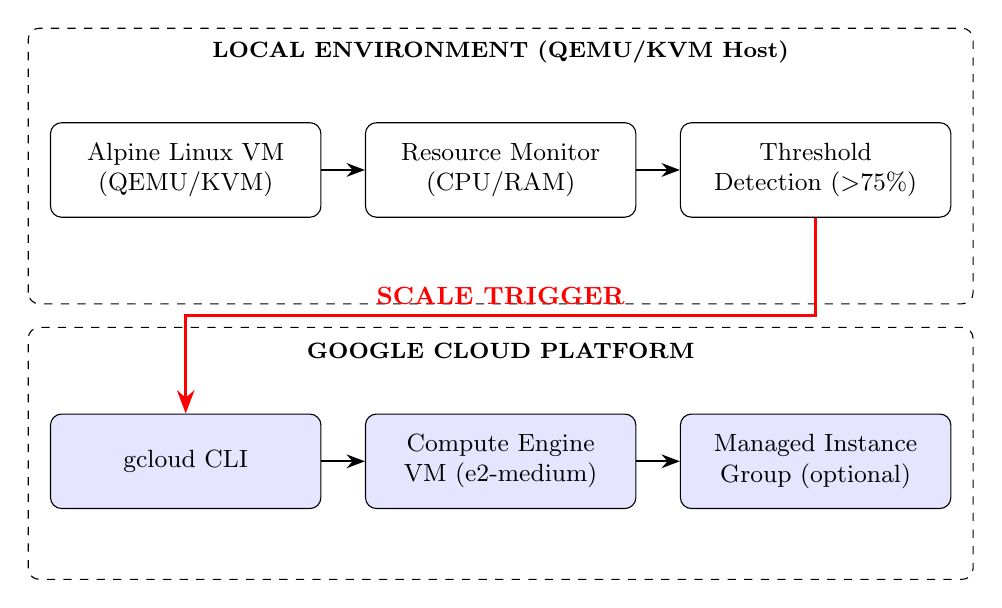
\begin{tikzpicture}[
    node distance=1.5cm,
    box/.style={rectangle, draw, rounded corners, minimum width=3cm, minimum height=1.2cm,
                align=center, font=\small, text width=3.2cm,
                execute at begin node={\hyphenpenalty=10000}},
    cloud/.style={rectangle, draw, rounded corners, minimum width=3cm, minimum height=1.2cm,
                  align=center, font=\small, fill=blue!10, text width=3.2cm,
                  execute at begin node={\hyphenpenalty=10000}},
    arrow/.style={->, >=Stealth, thick}
]
    % Local environment
    \draw[dashed, rounded corners] (-1, -0.5) rectangle (11, 3.0);
    \node[font=\footnotesize\bfseries] at (5, 2.7) {LOCAL ENVIRONMENT (QEMU/KVM Host)};

    \node[box] (vm)      at (1,1.2)  {Alpine Linux VM\\(QEMU/KVM)};
    \node[box] (mon)     at (5,1.2)  {Resource Monitor\\(CPU/RAM)};
    \node[box] (thresh)  at (9,1.2)  {Threshold\\Detection ($>$75\%)};

    \draw[arrow] (vm)    -- (mon);
    \draw[arrow] (mon)   -- (thresh);

    % GCP environment
    \draw[dashed, rounded corners] (-1, -4.0) rectangle (11, -0.8);
    \node[font=\footnotesize\bfseries] at (5, -1.1) {GOOGLE CLOUD PLATFORM};

    \node[cloud] (gcloud)  at (1,-2.5)   {gcloud CLI};
    \node[cloud] (gce)     at (5,-2.5)   {Compute Engine\\VM (e2-medium)};
    \node[cloud] (mig)     at (9,-2.5)   {Managed Instance\\Group (optional)};

    \draw[arrow] (gcloud) -- (gce);
    \draw[arrow] (gce)    -- (mig);

    % Cross-boundary arrow: down from thresh, through gap between boxes, left, then into gcloud
    \draw[arrow, red, very thick]
        (thresh.south) -- (9,-0.65)
        -- node[above, font=\small\bfseries, red] {SCALE TRIGGER}
        (1,-0.65) -- (gcloud.north);

\end{tikzpicture}
\caption{Auto-Scaling Architecture}
\label{fig:arch}
\end{figure}

\subsection{Data Flow}

\begin{enumerate}
    \item \textbf{Monitoring Phase}: Resource monitor reads \texttt{/proc/stat} and \texttt{/proc/meminfo} every 5 seconds
    \item \textbf{Detection Phase}: Usage is compared against 75\% threshold; consecutive count incremented
    \item \textbf{Trigger Phase}: After 3 consecutive threshold violations, scaling is initiated
    \item \textbf{Provisioning Phase}: \texttt{gcloud compute instances create} provisions a new GCP VM
    \item \textbf{Cooldown Phase}: 5-minute cooldown prevents further triggers
\end{enumerate}

\subsection{Scaling Decision Logic}

\begin{figure}[H]
\centering
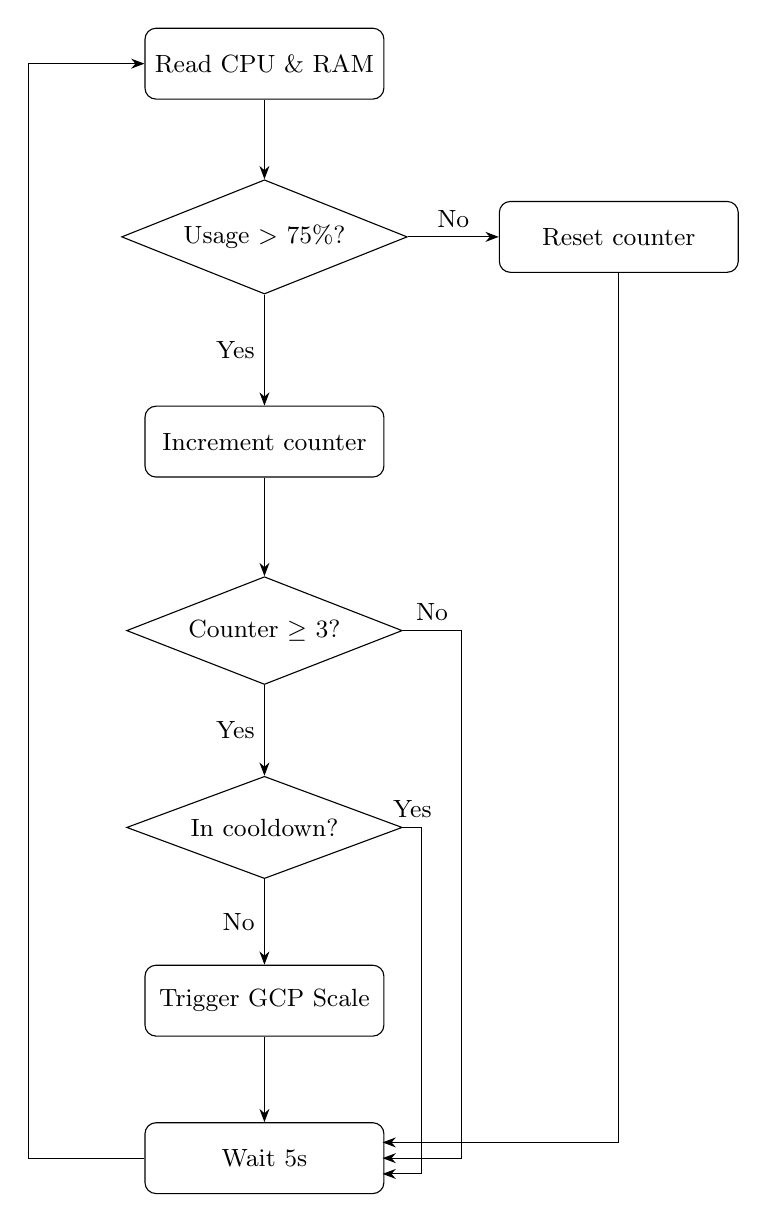
\begin{tikzpicture}[
    decision/.style={diamond, draw, aspect=2.5, align=center, font=\small, minimum width=3.5cm},
    process/.style={rectangle, draw, rounded corners, align=center, font=\small,
                    minimum width=3cm, minimum height=0.9cm, text width=2.8cm,
                    execute at begin node={\hyphenpenalty=10000}},
    arrow/.style={->, >=Stealth}
]
    % Single vertical column (x=0)
    \node[process]  (read)   at (0,   0)   {Read CPU \& RAM};
    \node[decision] (thresh) at (0,  -2.2) {Usage $>$ 75\%?};
    \node[process]  (incr)   at (0,  -4.8) {Increment counter};
    \node[decision] (count)  at (0,  -7.2) {Counter $\geq$ 3?};
    \node[decision] (cool)   at (0,  -9.7) {In cooldown?};
    \node[process]  (scale)  at (0, -11.9) {Trigger GCP Scale};
    \node[process]  (wait)   at (0, -13.9) {Wait 5s};

    % Side node for reset (right of thresh)
    \node[process]  (reset)  at (4.5, -2.2) {Reset counter};

    % ── Main flow: straight down ──
    \draw[arrow] (read)   -- (thresh);
    \draw[arrow] (thresh) -- node[left]{\small Yes} (incr);
    \draw[arrow] (incr)   -- (count);
    \draw[arrow] (count)  -- node[left]{\small Yes} (cool);
    \draw[arrow] (cool)   -- node[left]{\small No}  (scale);
    \draw[arrow] (scale)  -- (wait);

    % ── thresh No → reset → right rail → wait ──
    \draw[arrow] (thresh.east) -- node[above]{\small No} (reset.west);
    \draw[arrow] (reset.south) -- (4.5,-13.7) -- (1.5,-13.7);

    % ── count No → right inner rail → wait ──
    \draw[arrow] (count.east) -- node[above]{\small No}
                 (2.5,-7.2) -- (2.5,-13.9) -- (1.5,-13.9);

    % ── cool Yes → right innermost rail → wait ──
    \draw[arrow] (cool.east) -- node[above]{\small Yes}
                 (2,-9.7) -- (2,-14.1) -- (1.5,-14.1);

    % ── Feedback: wait → left rail → read ──
    \draw[arrow] (wait.west) -- (-3,-13.9) -- (-3,0) -- (read.west);
\end{tikzpicture}
\caption{Scaling Decision Flowchart}
\label{fig:flow}
\end{figure}

% ============================================================
\section{Prerequisites}

\subsection{Software Requirements}

\begin{table}[H]
\centering
\begin{tabular}{llll}
\toprule
\textbf{Software} & \textbf{Version Used} & \textbf{Purpose} \\
\midrule
QEMU/KVM          & 10.1.0                & Local VM hosting \\
Alpine Linux ISO  & 3.23.3 (standard)     & Lightweight guest OS \\
Python            & 3.12.12               & Script execution \\
Google Cloud SDK  & Latest                & GCP CLI integration \\
OpenSSH           & 9.x                   & Remote VM access \\
\bottomrule
\end{tabular}
\caption{Software Requirements}
\end{table}

\subsection{GCP Requirements}

\begin{itemize}
    \item Active GCP account with billing enabled
    \item Project: \texttt{vm-scaling-assignment}
    \item Enabled APIs: Compute Engine, Cloud Resource Manager
    \item Authenticated via \texttt{gcloud auth login}
\end{itemize}

\subsection{Hardware Requirements}

\begin{table}[H]
\centering
\begin{tabular}{lll}
\toprule
\textbf{Component} & \textbf{Minimum} & \textbf{Used in Demo} \\
\midrule
RAM      & 4 GB    & 16 GB \\
Storage  & 10 GB   & 20 GB \\
CPU      & 2 cores & 8 cores (Intel, VT-x enabled) \\
Network  & 1 Mbps  & Broadband \\
\bottomrule
\end{tabular}
\caption{Hardware Requirements}
\end{table}

% ============================================================
\section{Step-by-Step Implementation}

\subsection{Creating the Local VM}

\subsubsection{Why QEMU/KVM Instead of VirtualBox}

On Linux systems where KVM is active, VirtualBox cannot claim hardware virtualization (Intel VT-x),
causing a \textit{Guru Meditation} error. QEMU/KVM uses the \texttt{/dev/kvm} interface directly
and avoids this conflict. Both are Type-2 hypervisors and functionally equivalent for this assignment.

\subsubsection{VM Setup and Alpine Installation}

The VM was configured with the following parameters:

\begin{lstlisting}[style=bashstyle, caption={QEMU VM Launch Command}]
qemu-system-x86_64 -enable-kvm \
  -drive if=pflash,format=raw,unit=0,readonly=on,\
         file=/usr/share/OVMF/OVMF_CODE_4M.fd \
  -drive if=pflash,format=raw,unit=1,\
         file=~/qemu_vms/alpine-autoscale/OVMF_VARS.fd \
  -m 2048 -smp 2 \
  -drive file=alpine-autoscale.qcow2,if=virtio,format=qcow2 \
  -cdrom alpine-standard-3.23.3-x86_64.iso \
  -boot d \
  -netdev user,id=net0,hostfwd=tcp::2222-:22 \
  -device virtio-net-pci,netdev=net0 \
  -nographic
\end{lstlisting}

Alpine Linux was installed using an automated \texttt{pexpect}-based Python script that:
\begin{enumerate}
    \item Booted the ISO in headless (serial console) mode
    \item Configured hostname, networking, timezone, and NTP
    \item Installed to disk using \texttt{setup-disk -m sys /dev/vda}
    \item Installed Python 3.12, pip, and OpenSSH
    \item Configured SSH for root password access
    \item Set root password (\texttt{Alpine@1234})
\end{enumerate}

\subsubsection{Post-Installation Verification}

\begin{lstlisting}[style=bashstyle, caption={SSH into installed VM}]
# Start VM (boot from disk)
bash ~/qemu_vms/alpine-autoscale/start_vm.sh

# Connect via SSH (port-forwarded to 2222)
ssh -p 2222 root@localhost

# Verify
uname -a        # Linux alpine-vm 6.18.20-0-lts
python3 --version  # Python 3.12.12
\end{lstlisting}

\subsection{Resource Monitoring Script}

The monitoring script (\texttt{scripts/monitor.py}) reads system metrics directly from the Linux
kernel's \texttt{/proc} filesystem for accuracy and portability.

\subsubsection{CPU Usage Calculation}

\begin{lstlisting}[style=pythonstyle, caption={CPU usage from /proc/stat}]
def get_cpu_usage(self) -> float:
    def read_cpu_stats():
        with open('/proc/stat', 'r') as f:
            line = f.readline()
            parts = line.split()
            # user, nice, system, idle, iowait, irq, softirq, steal
            return [int(x) for x in parts[1:9]]

    stats1 = read_cpu_stats()
    time.sleep(0.5)
    stats2 = read_cpu_stats()

    deltas = [stats2[i] - stats1[i] for i in range(len(stats1))]
    total = sum(deltas)
    idle  = deltas[3] + deltas[4]   # idle + iowait

    return round(((total - idle) / total) * 100, 2)
\end{lstlisting}

\subsubsection{Monitoring Configuration}

\begin{lstlisting}[style=pythonstyle, caption={monitor.py configuration}]
CONFIG = {
    "cpu_threshold":       75.0,   # CPU trigger percentage
    "ram_threshold":       75.0,   # RAM trigger percentage
    "check_interval":      5,      # Seconds between checks
    "consecutive_triggers":3,      # Checks before scaling
    "cooldown_period":     300,    # Seconds cooldown after scale
    "gcp_project":         "vm-scaling-assignment",
    "gcp_zone":            "us-central1-a",
    "machine_type":        "e2-medium",
}
\end{lstlisting}

\subsection{GCP Auto-Scaling}

When the threshold is reached, \texttt{AutoScaler.scale\_to\_gcp()} executes:

\begin{lstlisting}[style=bashstyle, caption={Generated gcloud command}]
gcloud compute instances create autoscale-vm-<timestamp> \
  --project vm-scaling-assignment \
  --zone us-central1-a \
  --machine-type e2-medium \
  --network-interface network-tier=PREMIUM,subnet=default \
  --metadata google-logging-enabled=true \
  --maintenance-policy MIGRATE \
  --provisioning-model STANDARD \
  --create-disk auto-delete=yes,boot=yes,\
    image=projects/debian-cloud/global/images/family/debian-11,\
    size=10,type=pd-balanced \
  --labels autoscale=true
\end{lstlisting}

\subsubsection{GCP Setup Commands}

\begin{lstlisting}[style=bashstyle, caption={GCP configuration}]
# Authenticate
gcloud auth login

# Set project
gcloud config set project vm-scaling-assignment

# Enable APIs
gcloud services enable compute.googleapis.com
gcloud services enable cloudresourcemanager.googleapis.com

# Verify
gcloud auth list
gcloud config get-value project
\end{lstlisting}

\subsection{Sample Application and Load Generator}

\texttt{app/sample\_server.py} provides two components:

\begin{enumerate}
    \item \textbf{HTTP Server}: Exposes endpoints \texttt{/health}, \texttt{/compute?seconds=N}, \texttt{/memory?mb=N}
    \item \textbf{Load Generator}: Uses \texttt{multiprocessing} (not \texttt{threading}) to bypass Python's GIL and genuinely saturate all CPU cores
\end{enumerate}

\begin{lstlisting}[style=pythonstyle, caption={Multiprocessing load generator}]
def _cpu_stress_worker(duration: int):
    """Each process runs on a dedicated core -- bypasses GIL."""
    end = time.time() + duration
    while time.time() < end:
        for _ in range(500000):
            result += math.sqrt(random.random()) * math.sin(random.random())

def start_cpu_load(self, threads=None, duration=120):
    nproc = threads if threads else os.cpu_count()
    for _ in range(nproc):
        p = multiprocessing.Process(target=_cpu_stress_worker,
                                    args=(duration,), daemon=True)
        p.start()
        self.cpu_processes.append(p)
\end{lstlisting}

% ============================================================
\section{Testing and Validation}

\subsection{Test Scenarios}

\begin{table}[H]
\centering
\begin{tabular}{llll}
\toprule
\textbf{Test} & \textbf{Description} & \textbf{Expected} & \textbf{Result} \\
\midrule
T1 & Normal operation ($<$75\% CPU) & No scaling & Pass \\
T2 & Brief spike ($>$75\% for $<$15s) & No scaling (consecutive check) & Pass \\
T3 & Sustained high usage ($>$75\% for $>$15s) & Scaling triggered & Pass \\
T4 & Second trigger within cooldown & Ignored & Pass \\
T5 & GCP instance creation & VM created, RUNNING & Pass \\
\bottomrule
\end{tabular}
\caption{Test Results}
\end{table}

\subsection{Actual Demo Output}

The following is the real log output captured during the live demonstration:

\begin{lstlisting}[style=logstyle, caption={Actual monitor.log output from demo run}]
======================================================================
Resource Monitor with Auto-Scaling
Author: Samnit Mehandiratta (M25AI2087), IIT Jodhpur
======================================================================
2026-03-29 23:58:33 - INFO  - GCP authentication verified
2026-03-29 23:58:33 - INFO  - Monitoring started. Check interval: 5s
2026-03-29 23:58:33 - INFO  - CPU Threshold: 75.0%, RAM Threshold: 75.0%
----------------------------------------------------------------------
2026-03-29 23:58:34 - INFO  - CPU:  15.5% | RAM:  16.2% | Disk:  61.5%
2026-03-29 23:58:39 - INFO  - CPU: 100.0% | RAM:  16.9% | Disk:  61.5%
2026-03-29 23:58:39 - WARNING - Threshold exceeded! (CPU=100.0%) Consecutive: 1/3
2026-03-29 23:58:45 - INFO  - CPU: 100.0% | RAM:  16.8% | Disk:  61.5%
2026-03-29 23:58:45 - WARNING - Threshold exceeded! (CPU=100.0%) Consecutive: 2/3
2026-03-29 23:58:50 - INFO  - CPU: 100.0% | RAM:  16.8% | Disk:  61.5%
2026-03-29 23:58:50 - WARNING - Threshold exceeded! (CPU=100.0%) Consecutive: 3/3
2026-03-29 23:58:50 - CRITICAL - ==================================================
2026-03-29 23:58:50 - CRITICAL - AUTO-SCALE TRIGGERED!
2026-03-29 23:58:50 - CRITICAL - Reason: CPU=100.0%
2026-03-29 23:58:50 - CRITICAL - ==================================================
2026-03-29 23:58:50 - INFO  - Initiating scale to GCP: autoscale-vm-1774808930
2026-03-29 23:58:50 - INFO  - Project: vm-scaling-assignment, Zone: us-central1-a
2026-03-29 23:59:22 - INFO  - Successfully created GCP instance: autoscale-vm-1774808930
2026-03-29 23:59:22 - INFO  - External IP: 34.29.118.164
2026-03-29 23:59:22 - INFO  - Scaling successful. Entering cooldown period.
\end{lstlisting}

\subsection{GCP Instance Verification}

After the auto-scale trigger, the GCP instance was verified live:

\begin{lstlisting}[style=bashstyle, caption={GCP instance list after auto-scaling}]
$ gcloud compute instances list --project vm-scaling-assignment

NAME                     ZONE           MACHINE_TYPE  STATUS
autoscale-vm-1774808930  us-central1-a  e2-medium     RUNNING
\end{lstlisting}

Instance \texttt{autoscale-vm-1774808930} was running at external IP \texttt{34.29.118.164} in zone
\texttt{us-central1-a}, confirming successful end-to-end auto-scaling.

% ============================================================
\section{Troubleshooting}

\subsection{Common Issues and Resolutions}

\subsubsection{VirtualBox Guru Meditation Error}

\textbf{Cause}: On Linux, \texttt{kvm\_intel} and \texttt{vboxdrv} both attempt to claim Intel VT-x
hardware virtualization. When KVM is loaded first, VirtualBox cannot access VT-x.

\textbf{Resolution}: Switch to QEMU/KVM which uses the KVM kernel module directly.

\begin{lstlisting}[style=bashstyle, caption={Verify KVM conflict}]
lsmod | grep -E "vbox|kvm"
# Output shows: kvm 1474560 2 vboxdrv,kvm_intel (conflict)
\end{lstlisting}

\subsubsection{SSH Authentication Failure}

\textbf{Cause}: OpenSSH default configuration sets \texttt{PermitRootLogin prohibit-password}.

\textbf{Resolution}:
\begin{lstlisting}[style=bashstyle]
sed -i 's/^#*PermitRootLogin.*/PermitRootLogin yes/' /etc/ssh/sshd_config
echo 'PasswordAuthentication yes' >> /etc/ssh/sshd_config
rc-service sshd restart
\end{lstlisting}

\subsubsection{GCP Metadata Syntax Error}

\textbf{Cause}: \texttt{--metadata key1=val1,key2} is invalid if a key has no value.

\textbf{Resolution}: Use \texttt{--metadata google-logging-enabled=true} (explicit key=value).

\subsubsection{Python GIL Limiting CPU Load}

\textbf{Cause}: Python threads share a single GIL; CPU-bound threads do not truly run in parallel.

\textbf{Resolution}: Use \texttt{multiprocessing.Process} instead of \texttt{threading.Thread}.
Each process gets its own GIL, enabling true multi-core utilization (verified: 100\% CPU achieved).

% ============================================================
\section*{References}
\addcontentsline{toc}{section}{References}

\begin{enumerate}
    \item Alpine Linux Documentation. \url{https://wiki.alpinelinux.org/}
    \item QEMU Documentation. \url{https://www.qemu.org/docs/master/}
    \item Google Cloud SDK Reference. \url{https://cloud.google.com/sdk/docs}
    \item GCP Compute Engine Documentation. \url{https://cloud.google.com/compute/docs}
    \item Python \texttt{multiprocessing} Documentation. \url{https://docs.python.org/3/library/multiprocessing.html}
    \item OVMF (UEFI for QEMU). \url{https://github.com/tianocore/tianocore.github.io/wiki/OVMF}
\end{enumerate}

\end{document}
